\documentclass[11pt, oneside]{article} 
\usepackage{geometry}
\geometry{letterpaper} 
\usepackage{graphicx}
	
\usepackage{amssymb}
\usepackage{amsmath}
\usepackage{parskip}
\usepackage{color}
\usepackage{hyperref}

\graphicspath{{/Users/telliott/Github/figures/}}
% \begin{center} \includegraphics [scale=0.4] {gauss3.png} \end{center}

\title{Pentagons}
\date{}

\begin{document}
\maketitle
\Large

%[my-super-duper-separator]
In this chapter we explore some properties of a regular pentagon.  The pentagon has five-fold rotational symmetry.  Draw all of the internal chords of the figure and label a few angles.

By rotational symmetry each of the five vertices of the pentagon has the same three components, the central one labeled $s$, and two flanking ones $r$ and $t$.  
\begin{center}
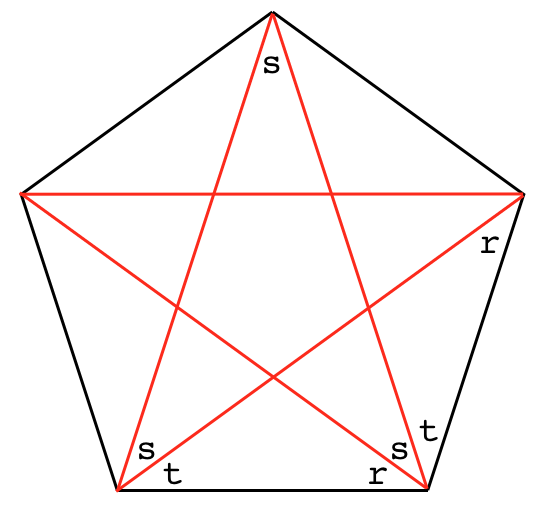
\includegraphics [scale=0.35] {pent1.png}
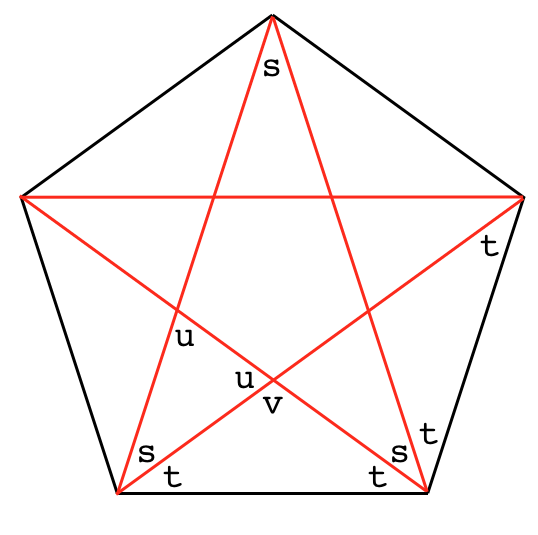
\includegraphics [scale=0.35] {pent2.png}
\end{center}
But $r = t$, by Thales' theorem, using two sides of the pentagon.  Hence we relabel, immediately (right panel).

We compute two triangle sums:
\[ 3s + 2t = 4t + s, \ \ \ \ \ 2s = 2t \]
Hence, $s = t$.  Relabel $t$ as $s$ (left panel, below):
\begin{center}
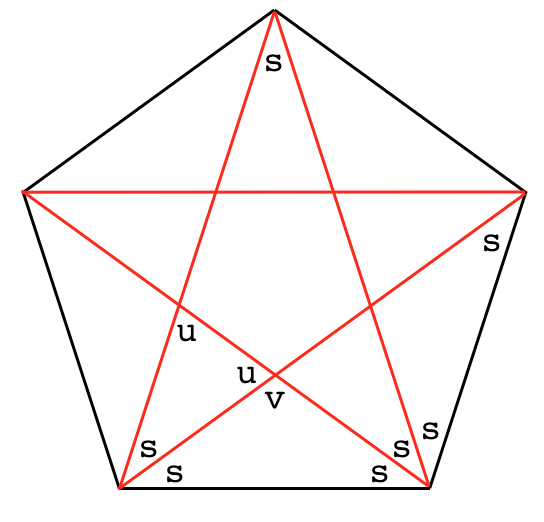
\includegraphics [scale=0.35] {pent3.png}
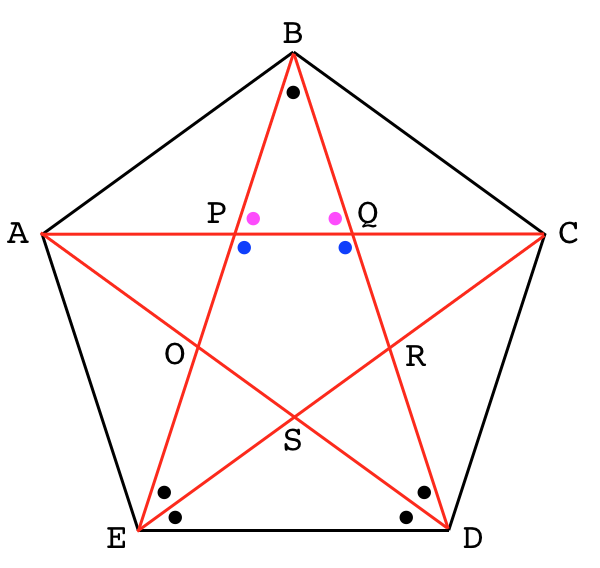
\includegraphics [scale=0.35] {pent4.png}
\end{center}
We observe that $5s = \pi$.
We again compute two triangle sums:
\[ 5s = v + 2s, \ \ \ \ \ v = 3s \]
\[ 5s = 2u + s, \ \ \ \ \ u = 2s \]

Since $v = 3s$, its measure is the same as the vertex angle of the pentagon.  Thus the inner figure is also a regular pentagon.

We do not need the angle labels any more, just the equalities.
\begin{center} 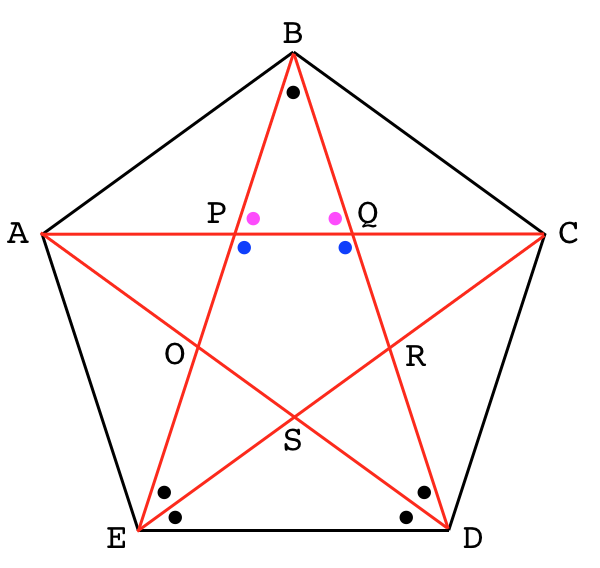
\includegraphics [scale=0.3] {pent4.png} \end{center}

$\triangle BED$ is similar to $\triangle BPQ$.  Hence the side of the inner pentagon is in the same measure to the side of the original pentagon as the ratio of $PQ$ to $AQ$.

Now observe that $AC$ is parallel to $ED$, because they have the equal alternate interior angles of two parallel lines.  (By similar triangles, or simply add the included angles).  Our drawing is filled with regular parallelograms, with four sides equal.

One can draw two types of isosceles triangles using the chords and sides of the pentagon.  One is tall and skinny, the other short and fat.  

The tall, skinny type have base angles equal to $s$.  Here are three examples:
\begin{center} 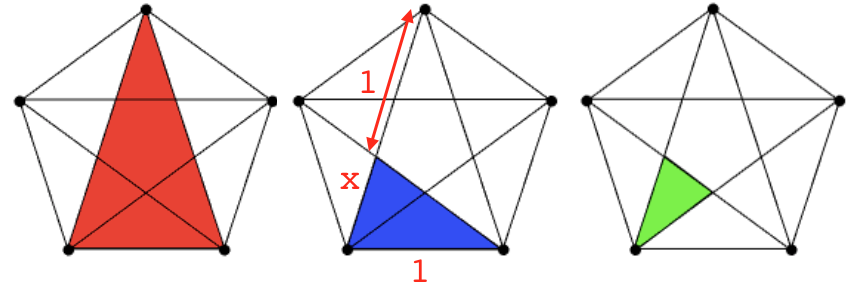
\includegraphics [scale=0.4] {three_triangles_2.png} \end{center}

If we take the side length of the original pentagon to be 1, then all the edges of regular parallelograms in the figure also have side length $1$, so the long side length of the red triangle is $1$ plus some other value, equal to the base of the blue triangle.  Let's call that extra part, $x$.  

We use the fact that red and blue are similar and form the ratio $\phi$ of the long side to the base (red on the left, blue on the right):
\[ \frac{1 + x}{1} = \frac{1}{x} \]
Rearrange:
\[ x^2 + x - 1 = 0 \]
\[ x = \frac{-1 \pm \sqrt{1 + 4}}{2} \]

Of course, $\phi$ is the golden ratio where we have taken the positive branch of the square root:
\[ \phi = 1 + x = \frac{1 + \sqrt{5}}{2} \]

From the similarity of the green triangle, if the side of the inner pentagon is $y$:
\[ \frac{x}{y} = \phi \]
\[ y = \frac{x}{1+x}  \]

\end{document}